Play the message signal using
\begin{lstlisting}
sudo apt install ffmpeg
ffplay fm/codes/msg/Sound_Noise.wav
\end{lstlisting}
\begin{enumerate}[label=\arabic*.,ref=\thesection.\theenumi]
\numberwithin{equation}{enumi}
\item Find the sampling rate of the message.
\\
	\solution
Executing	
\begin{lstlisting}
python3 fm/codes/msg/sample_rate.py
\end{lstlisting}
gives
the sampling rate of the input signal as 44100Hz.
\item Plot the spectrum of the message signal using the builtin FFT algorithm.\\
	\solution
The folowing code plots the spectrum in \figref{fig:FFTb} using the builtin FFT algorithm of the python library 'Numpy.'
\\
Executing
\begin{lstlisting}
python3 fm/codes/msg/msg_spec_amp.py
\end{lstlisting}		
\begin{figure}[H]
\centering
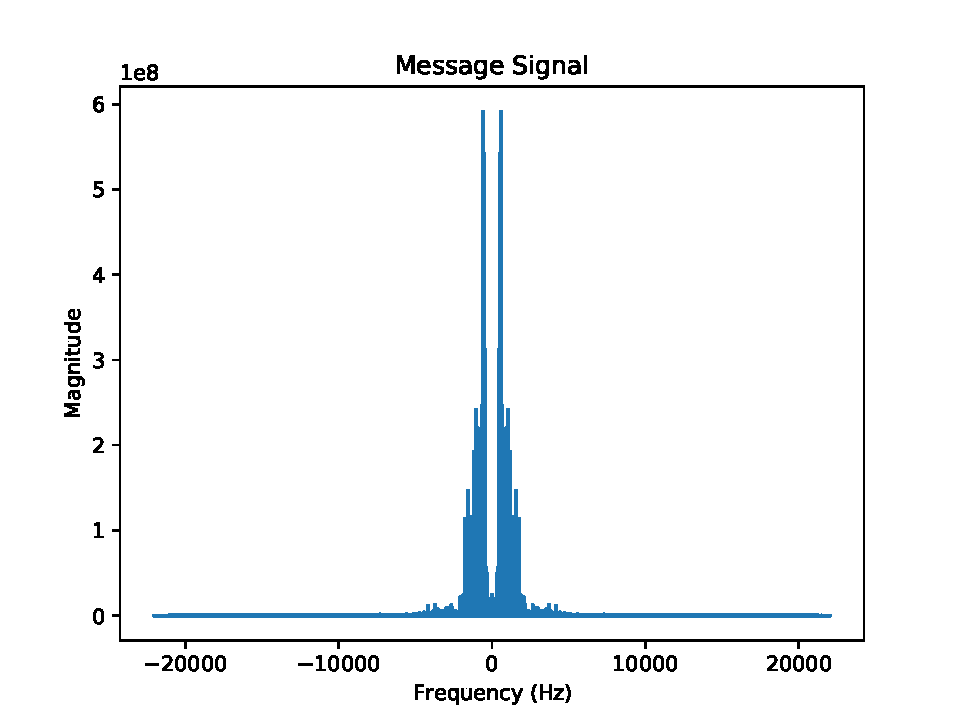
\includegraphics[width=\columnwidth]{fm/msg/figs/msg_spec_amp.pdf}
\caption{Plot of spectrum of message signal using builtin FFT algorithm.}
\label{fig:FFTb}
\end{figure}
\item Find the number of samples used to compute the FFT.\\
	\solution
The following code finds the number of samples used to compute the FFT
\begin{lstlisting}
python3 fm/codes/msg/no_of_samples.py
\end{lstlisting}
and gives number of samples as 1226536
\item What does the following command do?
\begin{lstlisting}
f_i = np.fft.fftfreq(len(audio_data), d=1/sample_rate)
\end{lstlisting}
The \textbf{np.fft.fftfreq} function divides the frequency range into equal intervals based on the sample rate and the number of samples. It returns an array of frequencies representing the DFT coefficients of the audio signal. These allow to analyze the spectrum of the audio signal in the frequency domain.
\item Plot the spectrum of the message signal by writing your own FFT algorithm.\\
	\solution
\begin{figure}[H]
\centering
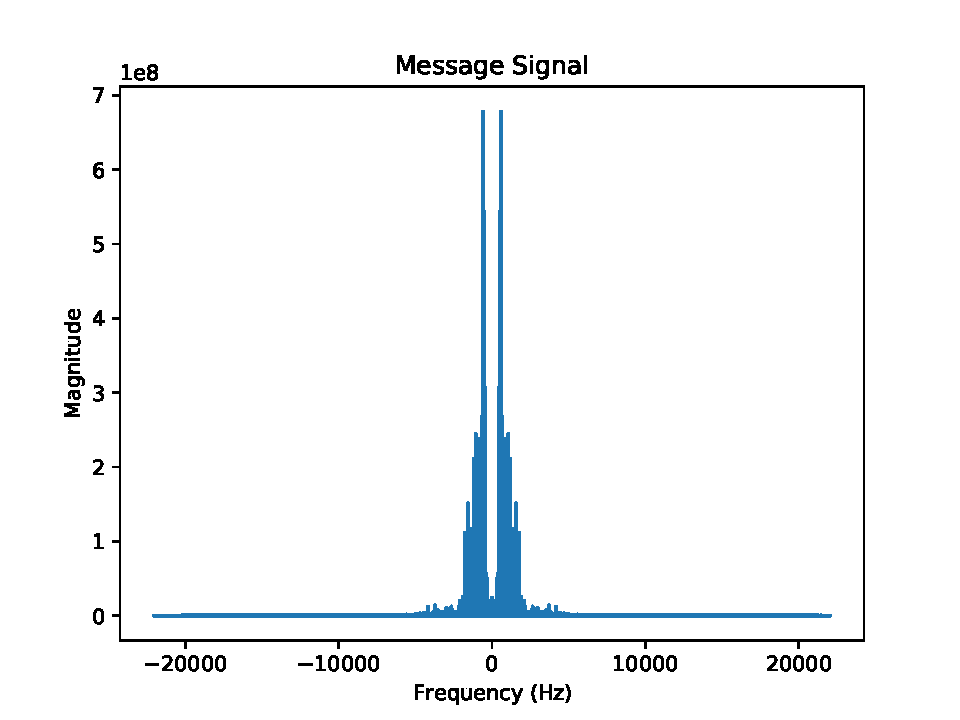
\includegraphics[width=\columnwidth]{fm/msg/figs/FFTmsg.pdf}
\caption{Plot of spectrum of message signal using own FFT algorithm.}
\label{fig:FFTo}
\end{figure}
The folowing code plots the spectrum in \figref{fig:FFTo} using the DFT defined in  \eqref{eq:app-dft-def}.
\begin{lstlisting}
python3 fm/codes/msg/FFTalgorithm.py
\end{lstlisting}
\item Compute and plot the PSD of the message signal using 
\eqref{eq:app-psd-def}.
\\
	\solution
Executing	
\begin{lstlisting}
python3 fm/codes/msg/msg_psd.py
\end{lstlisting}

\begin{figure}[H]
\centering
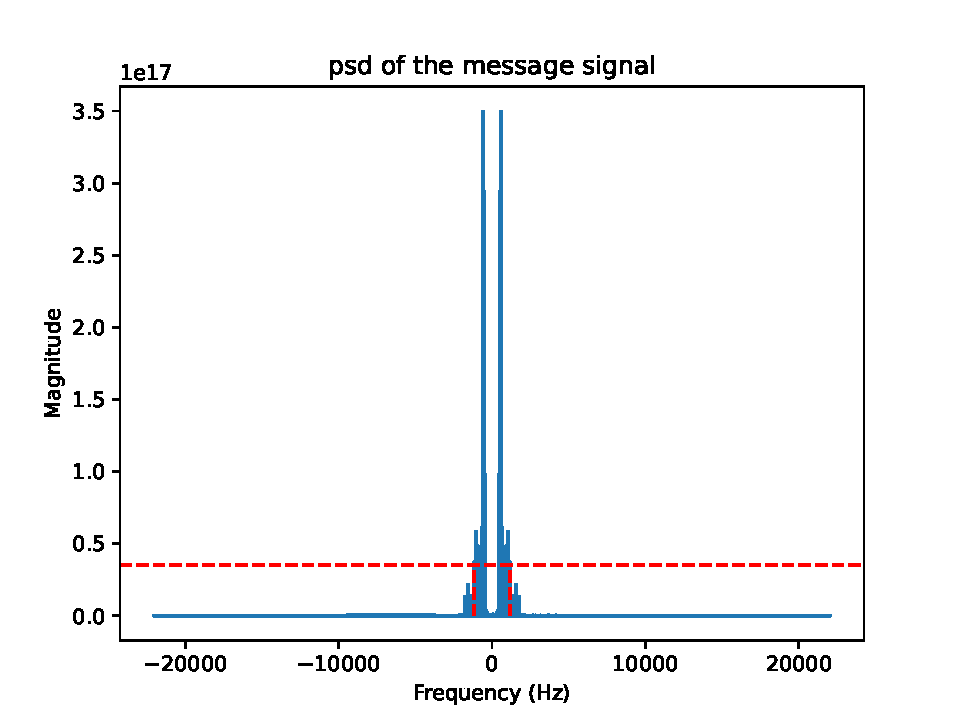
\includegraphics[width=\columnwidth]{fm/msg/figs/msg_psd.pdf}
\caption{Plot of PSD of the message signal.}
\label{fig:PSD}
\end{figure}

\item Find the bandwidth of the message signal.\\
\solution 
Executing
\begin{lstlisting}
python3 fm/codes/msg/msg_bw.py
\end{lstlisting}
gives the bandwidth of the message signal as 2366.625 Hz
\\
\iffalse
\begin{lstlisting}
/fm/codes/input.py
\end{lstlisting}
\fi

\end{enumerate}
